% siminos/gudorf/thesisProposal/proposal.tex
% $Author: mgudorf3 $ $Date: 2019-01-12 05:27:53 -0500 (Sat, 12 Jan 2019) $

%%%%%%%%%%%%%%%%%%%%%%%%%%%%%%%%%%%%%%%%%%%%%%%%%%%%%%%%%%%%%%%%%%%%%%
            \newif\ifpaper \newif\ifPDF \newif\ifboyscout
            %\newif\ifOUP \newif\ifdasbuch \newif\ifarticle
            %\newif\ifsolutions
            \boyscouttrue\PDFtrue\paperfalse
%%%%%% hyperlinked PDF version:
 \boyscouttrue  % commented, internal version
%  \boyscoutfalse % public
%%%%%% uncomment to generate paper B&W pdf for GaTech thesis submission:
%  \papertrue\boyscoutfalse

\documentclass[reqno,11pt,oneside]{article}

\usepackage[top=1in, bottom=1.2in, left=1.25in, right=1.25in]{geometry}
\usepackage[intlimits]{amsmath} % Puts the limits of integrals on top and bottom
\usepackage{amsxtra}     % Use various AMS packages
\usepackage{amsthm}
\usepackage{amssymb}
\usepackage{amsfonts}
\usepackage{ifthen}
\usepackage[font=small,labelfont=bf]{caption}
\usepackage{subcaption}
%%%%%%%%%%%%%%%%%%%%%%%%%%%%%%%%%%%%%%%%%%%%%%%%%%%%%%%%%%%%%%%%%%%%%%%%%%%%%%
\ifPDF %%%%%%%% HYPERLINKED VS PAPER PDF VERSIONS %%%%%%%%%%%%%%%%%%%%
   \usepackage[pdftex]{graphicx} % test switch to pdflatex?
  \ifpaper % prepare public B&W pdf individual chapters:
    \newcommand{\color}[1]{}
  \else    % prepare hyperlinked WWW/chapters/ChaosBook.pdf
    \usepackage[pdftex]{color}
            %% pdfmark produces Acroread index:
    \usepackage[pdfauthor={Matthew Gudorf}% must be LAST package loaded
                pdftitle={Just do it: Kuramoto-Sivashinsky state space},%
                pdftex,colorlinks]{hyperref} %% hyperlinks
            %% TEMPORARILY COMMENTED OUT backref:
    %       pdfmark,colorlinks,backref]{hyperref}
  \fi
%%%%%%%%%%%%%%%%%%%%%%%%%%%%%%%%%%%%%%%%%%%%%%%%%%%%%%%%%%%%%%%%%%%%%%%%%%%%%%


\graphicspath{{../../figs/ksstFigs/}
              {../../figs/}}

\newcounter{chapter}

\input{../../inputs/def}           %% do not edit; update from
\input{../../inputs/editsDasbuch}   %% editing comments, DasBuch style
\input{../thesis/defsThesis}
%%%%%%%%%%%%%%%%%%%%%%%%%%%%%%%%%%%%%%%%%%%%%%%%%%%%%%%%%%%%%%%%%%%%%%%%%%%%%%%
\begin{document}

\title{Spatiotemporal formulation of the Kuramoto-Sivashinsky equation}
\author{Matthew N. Gudorf}
\date{January 10, 2019} %{August 20, 2018}
\maketitle

\begin{abstract}


\documentclass[12pt]{article}
\usepackage{amsfonts}
\usepackage{amssymb}
\usepackage{authblk}
\usepackage{amsmath}

\newcommand{\KS}{Kuramoto-Siva\-shin\-sky}
\newcommand{\KSe}{Kuramoto-Siva\-shin\-sky equation}

\renewcommand\Authfont{\scshape\small}
\renewcommand\Affilfont{\itshape\small}
\setlength{\affilsep}{1em}

\newcommand{\smalllineskip}{\baselineskip=5pt}
\renewenvironment{abstract}[0]{\small\rm
        \begin{center}ABSTRACT
        \\ \vspace{2pt}
        \begin{minipage}{6.0in}\smalllineskip
        \hspace{1pc}}{\end{minipage}\end{center}\vspace{-1pt}}
\newcommand{\emailaddress}[1]{\newline{\sf#1}}

\let\LaTeXtitle\title
\renewcommand{\title}[1]{\LaTeXtitle{\large\textsf{\textbf{#1}}}}

%%%TITLE
\title{Lyapunov exponents, Floquet exponents and covariant vectors of \KSe}
\date{}

%%AFFILIATIONS
\author[1]{Xiong Ding}
\author[2]{Daniel Crane}
\author[1]{Predrag Cvitanovi\'{c}}
\author[2]{Ruslan L. Davidchack}
\author[3]{Kazumasa A. Takeuchi}
\affil[1]{School of Physics, Georgia Inst. of Technology,\emailaddress{xding@gatech.edu}}
\affil[2]{Dept. of Mathematics, Univ. of Leicester,
          Leicester LE1 7RH, UK}
\affil[3]{Dept. of Physics, Univ. of Tokyo, Japan}

%%DOCUMENT
\begin{document}
\maketitle

%%PLEASE PUT YOUR ABSTRACT HERE
\begin{abstract}
The largest positive Lyapunov exponent has long been used as an
indicator of chaotic dynamics, and recently sets of `covariant Lyapunov vectors'
have been shown to determine the `physical dimension' of a strange
attractor~\cite{GiChLiPo12} of a spatially extended flow,
for ex. the \KS\ on a finite periodic
domain. Such system can have a large range of Lyapunov
exponents, some
 expanding rapidly along the few unstable eigen-directions,
 while others contract dramatically along the many stable eigen-directions.
It
is a challenge to calculate those exponents accurately; the
\textit{QR iteration}~\cite{Trefethen97} provides a practical way to
evaluate them.
\\\\

The evolution of the tangent space of a dynamic system is governed by
the Jacobian matrix $\delta x(x_0, t)=J^t(x_0)\,\delta x(x_0, 0)$.
For a periodic orbit, the eigenvalues of the Jacobian matrix are called the
Floquet multipliers, and the associated Floquet eigenvectors
define the invariant directions
of the tangent space. The eigen-equation cannot be solved in
the traditional way, as the magnitude of matrix elements in such
Jacobian matrix can easily range over 100 orders of magnitude.
We show that the \textit{periodic Schur
decomposition}~\cite{Bojanczyk92theperiodic} enables us to compute
{\em all} eigenvalues to a high precision, provided the dimension
(the number of spatial Fourier modes) is not too high.



\end{abstract}
%%THE END OF ABSTRACT

\begin{thebibliography}{99}
\small
\bibitem{GiChLiPo12}
    F. Ginelli, H. Chat\'{e}, R. Livi and A. Politi,
  \textit{Covariant {Lyapunov} vectors}, J. Phys. A 46,
 2013, 254005.

\bibitem{Trefethen97} L. N. Trefethen and D. Bau, \textit{Numerical Linear
    Algebra}, SIAM, Philadelphia, 1997.

\bibitem{Bojanczyk92theperiodic} A. Bojanczyk, G. Golub and P. Van Dooren,
    \textit{The periodic Schur decomposition. Algorithms and
    applications}, In Proc. SPIE Conference, 1992, 31-42.

\end{thebibliography}
\end{document}

\end{abstract}

% siminos/xiong/thesis/chapters/intro.tex
% $Author: predrag $ $Date: 2021-06-22 07:16:06 -0400 (Tue, 22 Jun 2021) $

The study of nonlinear dynamics covers a huge range of research topics.
In this thesis, we focus on the geometric or topological structures and
statistic averages of dissipative systems. The progress in this area comes
from collaborative contributions from both applied mathematicians and
physicists, from both theoretical and numerical aspects.
In this chapter, we introduce the mathematical framework to study the
finite\dmn\ behavior embedded in an infinite\dmn\ function
space of dissipative systems described by nonlinear partial differential
equations (PDEs).
In particular, we review the recent progress in use of ``covariant vectors'' for
investigating the dimensionality of chaotic systems.
We also focus on the important role that invariant structures such as \po s
play in the description of chaotic dynamics and review the \emph{cycle averaging
theory}\rf{DasBuch} for calculating statistical properties of chaotic
dynamical systems.

% siminos/xiong/thesis/proposal/tex/done.tex
% $Author: predrag $ $Date: 2015-09-06 09:25:51 -0400 (Sun, 06 Sep 2015) $

\section{Preliminary results}
\label{sec:done}

\subsection{Computing \Fv s by \Ped}
\label{subsec:PE}

\begin{figure}[h]
  \centering
  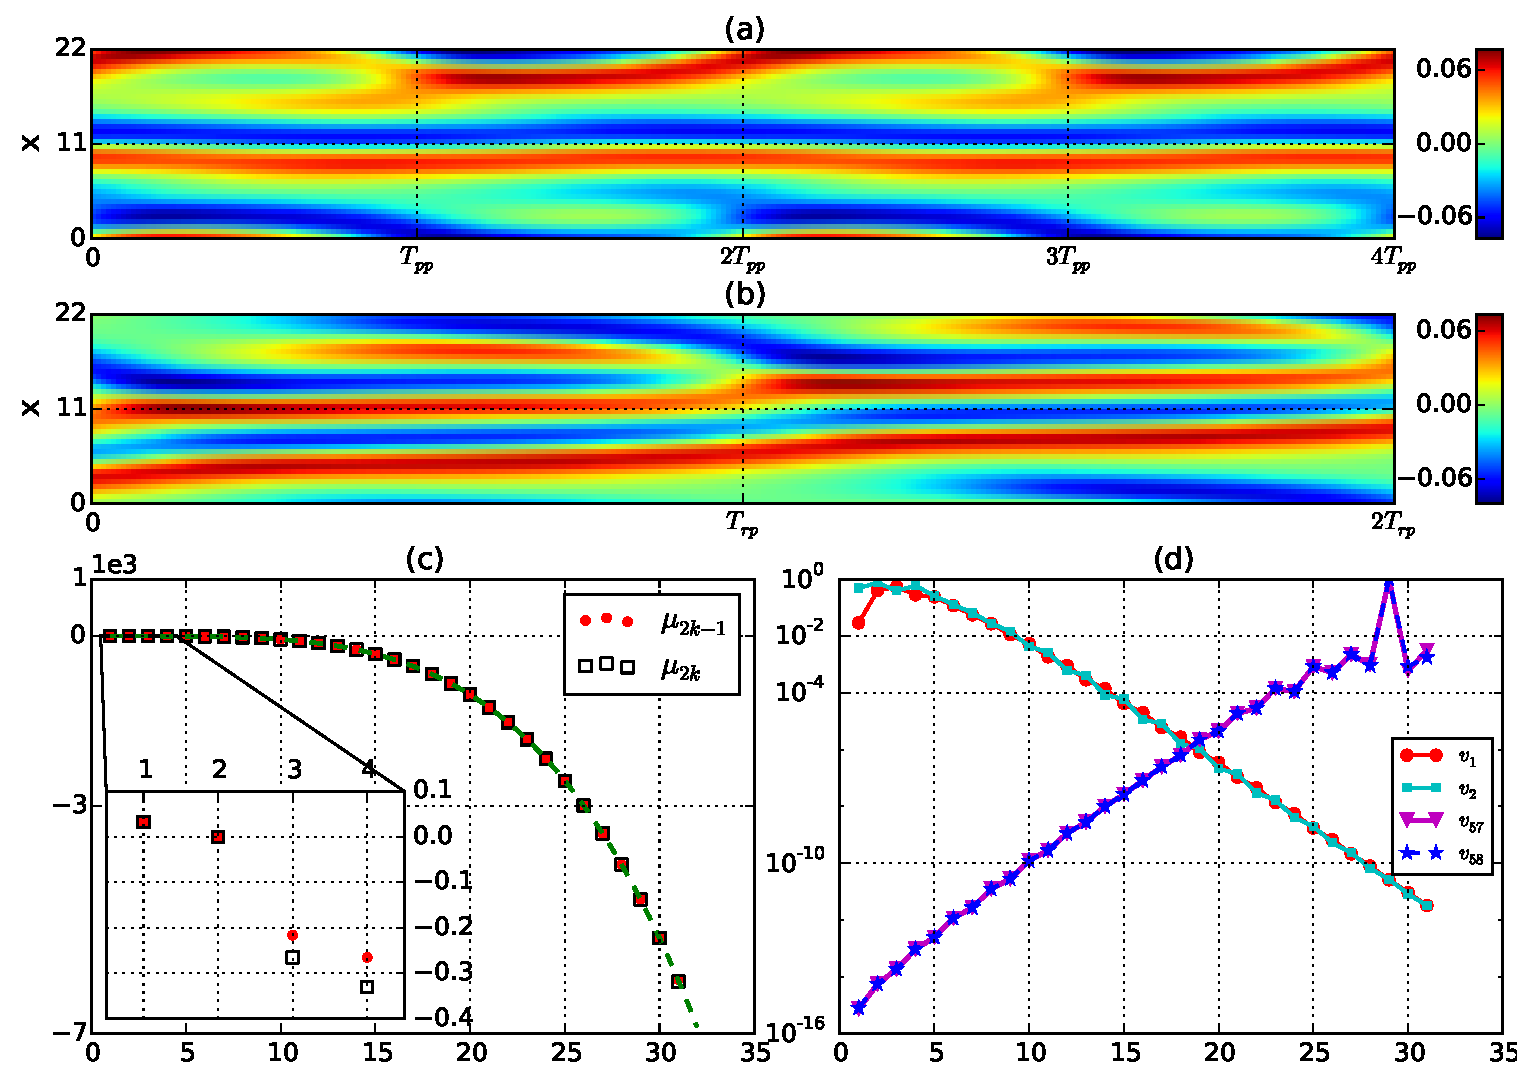
\includegraphics[width=0.9\linewidth]{pprpfigure}
  \caption{(Color online)
   (a) Pre\po\ $\cycle{pp}_{10.25}$ and
   (b) \rpo\ $\cycle{rp}_{16.31}$ in the full \statesp\ for total time
   $4\,\period{pp}$ and $2\,\period{rp}$, respectively. The phase shift
   for $\cycle{rp}_{16.31}$ after one prime period $\simeq-2.863$.
   (c) The real parts of Floquet exponents paired for a given $k$ as
   $(k,\eigRe[2k-1])$ and $(k,\eigRe[2k])$, for $\cycle{pp}_{10.25}$ with
   truncation number $N=64$. The dashed line (green) is
   $q_{k}^{2}-q_{k}^{4}$, with $x$-axis the indices of Fourier modes
   $k=1,2,\cdots,N/2-1$. The inset is a magnification of the region
   containing the 8 leading {\entangled} modes. As can be seen in
   \reftab{tab:floquet_ppo1}, for modes that follow, $k\geq 5$,
   the exponents are much smaller, in
   agreement with the expected separation into {\entangled} and
   {isolated} modes of \refref{YaTaGiChRa08}. For large
   indices, Floquet exponents
   appear in pairs corresponding to the real and imaginary
   part of Fourier modes.
   (d) The magnitudes of the Fourier components $|a_k| =
   |b_k+1i*c_k|$ of the 1st, the 2nd, the 57th and 58th \Fv s
   $\jEigvec[k]$ for $\cycle{pp}_{10.25}$ at initial time $\zeit =0$,
   truncation number $N=64$. For {\entangled} modes the first 4 Fourier
   are comparable in magnitude. For the $k_{th}$ isolated modes pair, the
   amplitude is concentrated on $k_{th}$ Fourier mode. The $x$-axis is
   labeled by the Fourier mode indices. Only the $k>0$ part is shown, the
   negative $k$ follow by reflection.
   }
  \label{fig:ppo1state}
\end{figure}

\begin{table}[h]
  \footnotesize
  \centering
  \caption{
    The first 10 and last four Floquet exponents and
    Floquet multiplier phases,
    $ \ExpaEig_i= \exp(\period{}\,\eigRe[i] \pm i\theta_{i})$, for
    orbits $\cycle{pp}_{10.25}$ and $\cycle{rp}_{16.31}$, respectively.
    $\theta_{i}$ column lists either the phase,
    if the Floquet multiplier is complex, or `-1' if the
    multiplier is real, but inverse hyperbolic. Truncation number
    $N=64$.
    The $8$ leading exponents correspond to the {\entangled} modes:
    note the sharp drop in the value of the $9_{th}$ and subsequent
    exponents, corresponding to the {isolated} modes.
  }
  \label{tab:floquet_ppo1}
  \begin{tabular}{l l c | l l c}
    \multicolumn{3}{c |}{$\cycle{pp}_{10.25}$} & \multicolumn{3}{c}{$\cycle{rp}_{16.31}$}\\
    $i$ & ~~~~~$\eigRe[i]$  & $\theta_{i}$  & $i$ & ~~~~~$\eigRe[i]$ & $\theta_{i}$  \\
    \hline
    1,2 & ~0.033209  &    $\pm$2.0079  &  1 &     ~0.32791  &              \\
    3 & -4.1096e-13  &                 &  2 &   ~2.8679e-12  &              \\
    4 & -3.3524e-14  &    -1           &  3 &   ~2.3559e-13  &              \\
    5 &  -0.21637    &                 &  4 &     -0.13214  &        -1    \\
    6,7 &  -0.26524  &   $\pm$2.6205   &  5,6 &   -0.28597  & $\pm$2.7724  \\
    8 &  -0.33073    &    -1           &  7 &     -0.32821  &       -1     \\
    9 &  -1.9605    &                  &  8 &      -0.36241  &             \\
    10 & -1.9676    &    -1            &  9,10 &   -1.9617  &  $\pm$2.2411 \\
    $\cdots$ &  $\cdots$    & $\cdots$ & $\cdots$ & $\cdots$ & $\cdots$   \\
    59 &  -5313.6   &    -1           &  59 &   -5314.4 &                 \\
    60 &  -5317.6   &                 &  60 &   -5317.7 &                 \\
    61 &  -6051.8   &    -1           &  61 &   -6059.2 &                 \\
    62 &  -6080.4   &                 &  62 &   -6072.9 &                 \\
    \hline
\end{tabular}
\end{table}
\begin{figure}[h]
  \centering
  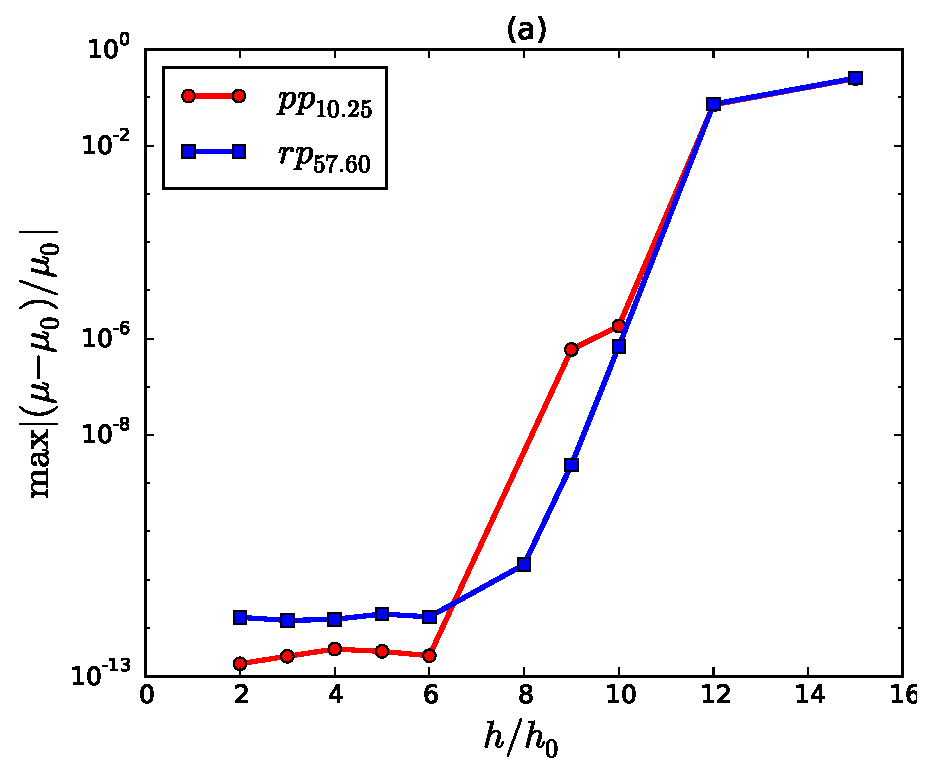
\includegraphics[width=0.47\linewidth]{ppo1FEerror} \hfill
  \includegraphics[width=0.47\linewidth]{rpo22FEerror}
  \caption{(Color online) Relative error of the real part of
    Floquet exponents associated with different time steps
    with which the Floquet matrix is integrated. Two orbits $\cycle{pp}_{10.25}$
    and $\cycle{rp}_{57.60}$ are used as an example with the base
    case $h_0 \approx 0.001$. (a) The maximal relative difference of
    the whole set of Floquet exponents with increasing time step (decreasing
    the number of ingredient segments of the orbit). (b) Only consider
    the first 35 Floquet exponents.}
  \label{fig:FEerror}
\end{figure}
\begin{figure}[h]
  \centering
  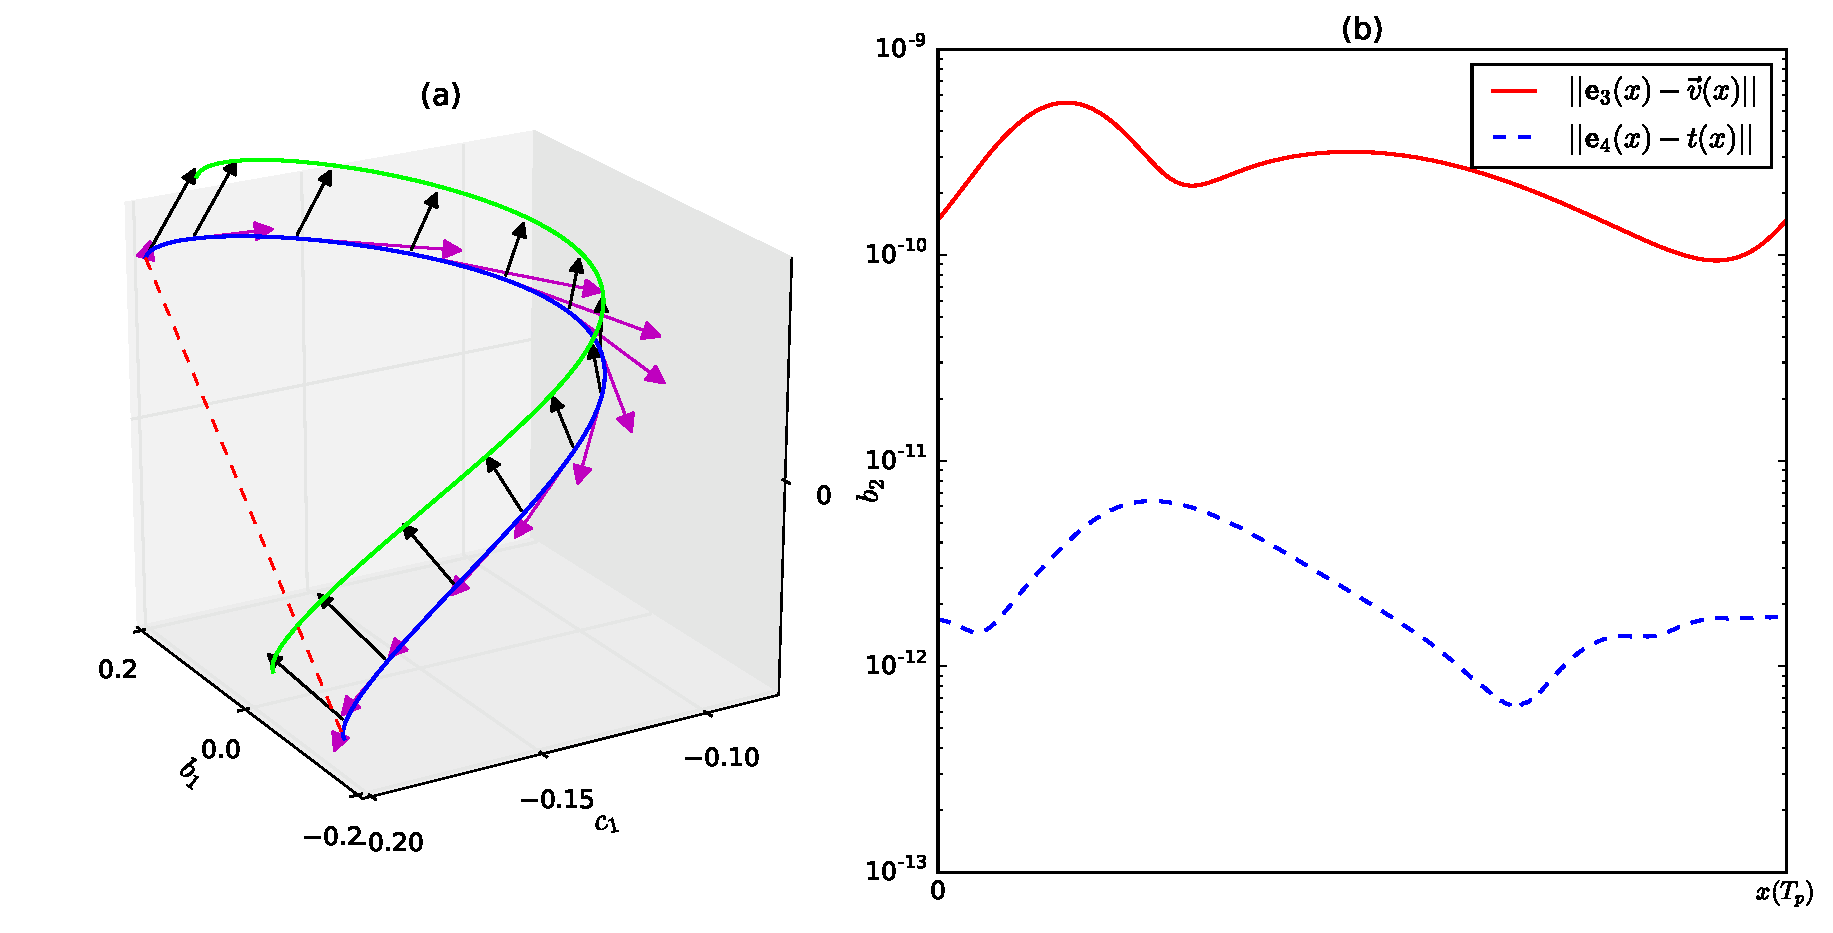
\includegraphics[width=1.0\linewidth]{ppo1vectfield}
  \caption{(Color online)
    Marginal vectors and the associated errors.
    (a) $\cycle{pp}_{10.25}$ in one period projected onto $[a_{1},b_{1},a_2]$
    subspace (blue curve), and its counterpart (green line) generated by
    a small group transformation $g(\ell)$
    , here arbitrarily set to $\ell= \,L/(20\pi)$. Magenta and black
    arrows represent the first and the second marginal \Fv s
    $\jEigvec[3](x)$ and $\jEigvec[4](x)$ along the prime orbit.
    (b) The solid red curve is the magnitude of the difference between
    $\jEigvec[3](x)$ and the velocity field $\vec{v}(x)$ along the orbit,
    and blue dashed curve is the difference between $\jEigvec[4](x)$ and
    the group tangent $t(x)=\mathbf{T}x$.
  }
  \label{fig:ppo1vectorfield}
\end{figure}


Stability analysis of \eqva\ is crucial for understanding the the geometry of
state space\rf{guckb}, but it is difficult for unstable \po s
due to lack of efficient and accurate numerical algorithms.
Floquet theorem says that
the Floquet matrix evaluated along a \po\ can be decomposed
as a product of a periodic matrix and an exponential matrix. We are interested
in the eigenvalues (Floquet multipliers) and the corresponding eigenvectors
(\Fv s) of the exponential matrix. More specifically,
define a flow $x(t) = f^t(x(0))$ generated by velocity field $\dot{x} = v(x)$
with $x$ a state vector. The evolution of perturbation along any orbit
is governed by the Jacobian of this flow
$J^t(x) = \partial f^t(x) / \partial x$, that is
$\delta x(t) = J^t(x) \delta x(0) $, and Jacobian itself is evolved as follows,
\begin{equation}
  \label{eq:jacobian}
  \frac{dJ^t(x)}{dt} = A(x)J^t(x)\,,\quad A(x) = \frac{v(x)}{x}
  \,.
\end{equation}
For a \po\ $x(T_p)=x(0)$,
the solution of \eqref{eq:jacobian}
for one period  $J_p = J^T(x(0))$ is called Floquet matrix or monodromy matrix.
$J_p e_i = e^{T(\eigRe[i]+\eigIm[i])} e_i$ gives the average expansion/contraction
rate $\eigRe[i]$ and
invariant directions $e_i$ in the tangent space.

For high dimensional nonlinear systems, Floquet exponents usually span a large
number of orders, so one period integration of \eqref{eq:jacobian} usually
results in a highly ill-conditioned Jacobian matrix, so we need to conduct
transformations on each short-time Jacobian since whole matrix can be decomposed
into the product of a sequence of square matrix. This is the basic idea of
\emph{\ped}, and it is based on the idea on \cLv\ algorithm and
\psd\ algorithm introduced in sec.~\ref{subsec:CAPSD}. See
\rf{DingCvit14} for the implementation details. Here, we only show the result
with 1-dimensional \KSe\ defined on a periodic domain.
\begin{equation}
u_t+\frac{1}{2}(u^2)_x+u_{xx}+u_{xxxx}=0\,,\; x\in [0,L]
\label{eq:ks}
\end{equation}
Here domain size $L=22$.
\KSe\ is equivariant under reflection and space translation: $-u(-x,t)$ and
$u(x+l,t)$ are also solutions if $u(x,t)$ is a solution.
Based on the consideration of these symmetries,
we focus on two types of orbits:
pre\po s $\hat{u}(0)=R\hat{u}(\period{p})$  and \rpo,
$\hat{u}(0)=g_p\hat{u}(\period{p})$. Here $R$ and $g_p$ are reflection and
rotation respectively.

At each repeat of the prime period, $\cycle{pp}_{10.25}$ is invariant
under reflection along $x=L/2$, \reffig{fig:ppo1state}\,(a), and
$\cycle{rp}_{16.31}$ has a shift along the $x$ direction as time goes on,
\reffig{fig:ppo1state}\,(b). Since $\cycle{pp}_{10.25}$ and
$\cycle{rp}_{16.31}$ are both
time invariant and equivariant under SO(2) group transformation $g(l)$,
there should be two marginal Floquet exponents, corresponding to the
velocity field and group tangent respectively.
\refTab{tab:floquet_ppo1} shows that the $2_{nd}$ and $3_{rd}$,
respectively $3_{rd}$ and $4_{th}$ exponents of $\cycle{rp}_{16.31}$,
respectively $\cycle{pp}_{10.25}$, are marginal, with accuracy as low as
$10^{-12}$, to which the inaccuracy introduced by the error in the closure of
the orbit itself also contributes.

In practice, caution should be
exercised when trying to determine the optimal number of time increments
that the orbit should be divided into. Here we determined satisfactory $m$'s by numerical
experimentation shown in \reffig{fig:FEerror}. Since larger time step means
fewer time increments of the orbit, a very small time step ($h_0 \approx 0.001$)
is chosen as the base case, and it is increased to test whether the
corresponding Floquet exponents change substantially or not. As shown in
\reffig{fig:FEerror} (a), up to $6h_0$ the whole Floquet spectrum varies within
$10^{-12}$ for both $\cycle{pp}_{10.25}$ and $\cycle{rp}_{57.60}$. These
two orbits represent two different types of invariant solutions which have
short and long periods, so we presume that time step $6h_0$ is good enough
for other short or long orbits too. On the other hand, if only the first
few Floquet exponents are desired, the time step can be increased further
to fulfill the job. As shown in \reffig{fig:FEerror} (b), if we are only
interested in the first 35 Floquet exponents, then time step $30h_0$ is small
enough. In high dimensional nonlinear systems, dynamics in the very contracting
directions is, very the often, decoupled from the physical modes, and shed little
insight into the system properties, so large time step could to used in order to
save time.
\refTab{tab:floquet_ppo1} and
\reffig{fig:ppo1state}\,(c) show that \psd\ is capable of resolving
Floquet multipliers differing by thousands of orders:
when $N=64$, the smallest Floquet multiplier  for $\cycle{pp}_{10.25}$ is
$|\ExpaEig_{62}| \simeq e^{-6080.4\times 10.25}$.

The two marginal directions have a simple geometrical interpretation.
\refFig{fig:ppo1vectorfield}\,(a) depicts the two marginal vectors of
$\cycle{pp}_{10.25}$ projected onto the subspace spanned by $[a_1, b_{1}, a_{2}]$
(the real, imaginary parts of the first mode and the real part of the
second Fourier mode). The first marginal eigen-direction (the $3_{rd}$
\Fv\ in  \reftab{tab:floquet_ppo1}) is aligned with the velocity
field along the orbit, and the second marginal direction (the $4_{th}$
\Fv) is aligned with the group tangent. The numerical
difference between the unit vectors along these two marginal directions
and the corresponding physical directions is shown in
\reffig{fig:ppo1vectorfield}\,(b). The difference is under $10^{-9}$ and
$10^{-11}$ for these two directions, which demonstrates the accuracy of
the algorithm.



\subsection{Local description of inertial manifold by \Fv s}
\label{subsec:LDIM}
Dissipative nonlinear systems described by partial differential equations
are infinite dimensional in principle, but for a lot of them, there exists
a finite dimensional inertial manifold and the dynamics is contained in it
after a transient period of evolution. Here we try to explain the concept of
``\emph{slaving}'' to understand how transition from infinite dimensional
space into finite dimensional subspace happens. For strict
mathematical treatment, see\rf{ Robinson1995, infdymnon}. Let $u$ be a dynamical
system in a finite or infinite dimensional Hilbert space $H$ governed by
\begin{equation}
  \label{eq:proto}
  \frac{du}{dt} + Au + f(u) = 0
\end{equation}
Assume this system has a n-dimensional inertial manifold, and
denote the projection from $H$ to the first $n$ eigenvectors of $A$ by
$P$. Let $Q = I - P$, then project \eqref{eq:proto} onto this subspace,
we obtain
\begin{equation}
  \label{eq:projected}
  \frac{dp}{dt} + Ap + Pf(p+\Phi(p)) = 0
\end{equation}
Here $p = Pu$ and $\Phi:PH\mapsto QH$. So we have reduced the dynamics to
a subspace given the existence of such a mapping $\Phi$, and the graph
of $\Phi$ is the inertial manifold. Equation \eqref{eq:projected} is
called the \emph{inertial form} of this system. Essentially, the existence
of inertial manifold indicates that the eigenmodes of $A$ with index larger than
$n$ is slaved to its first $n$ eigenmodes. For example, in \KSe,
eigenmodes of $A$ are Fourier modes, so short waves are slaved to long waves.
Anyway, inertial manifold can be interpreted in different ways, but the essential
idea is similar. See\rf{man90b} for an adiabatic illustration by a simple two
variable system.

To Approximate inertial manifold, or equivalently, to approximate
mapping $\Phi:PH\mapsto QH$ requires the knowledge of its exact dimension.
At present, people use empirical or some test number to truncate the
original system. For example, in \rf{foias88}, 3 modes are
used to represent the inertial manifold of 1-dimensional \KSe, but this
truncated model is not enough to preserve the bifurcation diagram. On the other
hand, mathematical upper bound for the dimension is not always tight.
However, as stated in
sec.~\ref{subsec:IM}, Recent progress in the numerical algorithm of \cLv s enables us
to expand tangent spaces into invariant subspaces.
\CLv s computed along long ergodic
trajectories are disentangled between the physical subspace and the transient
subspace, which serves as a criteria for determining the effective dimension
of the state space. This approach is different from the nonlinear Galerkin method
since it has no ambition to use a static set of eigenvectors to describe the dynamics,
it uses invariant vectors in the tangent space to linearly approximate the
inertial manifold locally.
From our intuition, we expect \Fv s along \po s can give the same dimension
of inertial manifold as \cLv s. Moreover, \Fv s seem more suitable for this job.
First, we have an efficient and accurate algorithm for calculating \Fv s
introduced in sec~\ref{subsec:PE}, and do not
need to follow an ergodic trajectory for a long time as \cLv\ algorithm does.
Second, \po s are dense on the strange attractor and probably only a
small subset of them is enough to represent the whole hierarchy in the system
if the symbolic dynamics of this system is known, so
experiments can be restricted to small number of short \po s.
But \cLv s along ergodic trajectories reveals little information about the
geometry of the strange attractor.


\paragraph{Angle distribution between physical and transient subspaces}
Like the experiments conducted in\rf{TaGiCh11, YaTaGiChRa08}, we measure the
angle between subspaces spanned by disjoint \Fv s along \po s inside
the 1-dimensional \KSe\ with domain size $L=22$.
Since symbolic dynamics in this system is unknown, we choose to do the statics
for all the \po s available to us with period $T<120$.
\begin{figure}[h]
  \centering
  \includegraphics[width=0.48\textwidth]{angle120ppoSpace1} \hfill
  \includegraphics[width=0.48\textwidth]{angle120rpoSpace1}
  \caption{Angle distribution $\rho(\theta)$ versus $\theta$
    for \cycle{ppo} (left) and \cycle{rpo} which has $ T < 120$.
  }
  \label{fig:angDist}
\end{figure}
As shown in \reffig{fig:angDist}, we are measuring the distribution of
the angle between invariant subspace spanned by the first $k$ \Fv s
and the subspace spanned the
remaining $30-k$ \Fv s. Start from $k=1$, As we add more into
the first subspace, the possibility keeps nonzero until $k = 9$, and after
which, the distribution shrinks away from zero. The same qualitative
distribution is obtained for both pre-\po s and \rpo s.
Therefore, the first 8 \Fv s are entangled with each other and are
disentangled from the remaining set. We call the first set physical
\Fv s and the latter unphysical one. The unphysical set has little effect
on the dynamics in the neighborhood of this \po\ since all theses directions
are contracting, and thus small perturbation inside it will die out eventually.
So clearly, the first 8 \Fv s are enough to approximate the inertial manifold
at the neighborhood of all the \po s concerned in this
experiment and we expect that such threshold number
will not
change if we can find more \po s.
Since \po s are dense on the attractor, we expect the same number
apply to the whole inertial manifold.

\paragraph{difference vectors spanned by subset of \Fv s}
Ergodic trajectories are attracted by \po s along their stable directions,
and repelled by their unstable directions. Each unstable direction is
important since it determines how the system is stretched; however, if the
inertial manifold exists, then only a subset of the stable directions
have an effect on the dynamics asymptotically. So we believe that an ergodic
trajectory is moving in a subspace which is spanned by the set of
all unstable \Fv s and a subset of stable \Fv s around a \po\ locally.
So, the number of \Fv s used to span such a subspace can be regarded
as the dimension of inertial manifold.
\begin{figure}[h]
  \centering
  \includegraphics[width=0.48\textwidth]{ppo3truncated} \hfill
  \includegraphics[width=0.48\textwidth]{rpo4truncated}
  \caption{
    scatter plot of $sin\theta$ vs the norm of difference vector.
    $\theta$ is the angle between $\Delta x$ and the subspace spanned
    by a subset of \Fv s.
    (a) $\cycle{ppo}_{32.36}$ with 198 shadowing incidences.
    (b) $\cycle{rpo}_{34.64}$ with 230 shadowing incidences.
  }
  \label{fig:angApproach}
\end{figure}

We borrow the idea from\rf{YaRa11} and conduct a set of experiments.
We generate a long ergodic trajectory and try to find incidences that it shadows
a specific \po. For each shadowing point $x$ on the ergodic trajectory,
we locate the nearest point $x_p$ on the \po\ to it and defined the
difference vector by $\Delta x = x - x_p$. When the orbit approaches or leaves the
\po, the difference vector is mainly controlled by the stable and unstable \Fv s,
so if we try to expand $\Delta x$ using a subset of \Fv s and see
how many of \Fv s is enough for a faithful expansion, we could almost get a
faithful approximation of the inertial manifold locally. In
\reffig{fig:angApproach}, if more than 7 \Fv s are used, then the
tendency shows that $\theta$ will
diminish to zero linearly as $\Delta x$ goes to zero, which is not true
if no more than 6 \Fv s are used to span the subspace. Note the experiments are
conducted in the symmetry-reduced state space, so the dimension of inertial
manifold of the full state space is $7+1$, which is consistent with the previous
result.

\subsection{Traveling wave in \cqcGLe}
In \cqcGL\ \eqref{eq:cqcgl1d}, traveling wave (\reqv) is defined as
a solution of
\[
A(x, 0) = e^{i\phi}A(x+ct, t)
\]
which is
\begin{equation}
  a_k(0) = e^{i\omega_\rho t}e^{ik\omega_\tau t}a_k(t)
  \label{eq:travelWaveFourier}
\end{equation}
in Fourier space.
Here $\omega_\rho$ is the velocity in the group tangent of phase
invariance symmetry: $\phi = \omega_\rho t$, and $\omega_\tau= 2\pi/L\cdot c$.
Levenberg-Marquardt algorithm is implemented to solve \eqref{eq:travelWaveFourier}
with random initial conditions. Dozens of {\reqva} are founded and a few
are shown in \reffig{fig:cqcglReqSet}.
Some of them are extensive spanning the whole domain; others are localized.
\begin{figure}[h]
  \centering
   (1)\includegraphics[width=.19\textwidth]{cqcglReq1T90}
   (2)\includegraphics[width=.19\textwidth]{cqcglReq2T90}
   (3)\includegraphics[width=.19\textwidth]{cqcglReq3T90}
   (4)\includegraphics[width=.19\textwidth]{cqcglReq4T90}\\
   (5)\includegraphics[width=.19\textwidth]{cqcglReq5T90}
   (6)\includegraphics[width=.19\textwidth]{cqcglReq6T90}
   (7)\includegraphics[width=.19\textwidth]{cqcglReq7T90}
   (8)\includegraphics[width=.19\textwidth]{cqcglReq8T90}
  \caption{
    A set of different relative \eqva. (1) is different from
    (7) by the phase velocity. Plane wave solutions like (2) appear
    most frequently, and there is a set of solutions like (2) with
    different phase velocities and translational velocities.
    Only one representative is shown here.
  }
  \label{fig:cqcglReqSet}
\end{figure}
Here I are only interested in the one related to the soliton
(1) shown in
\reffig{fig:req1Config}. This {\reqv} has group velocity
$\omega_\tau = 0$ and $\omega_\rho=17.6675$.
\refFig{fig:req1Config} shows the profile of this \reqv\ and
its stability exponents. \refTab{tab:req1Stability} gives
the numerical values of these exponents.
\begin{table}
  \centering
  \begin{tabular}{c | c}
    index & $\lambda$ \\
    \hline
     1,2    &    0.1474653 $\pm$      17.2375582i\\
     3,4    &    0.1474643 $\pm$      17.2375572i\\
     5    &    -7.21620620e-14             \\
     6    &     -1.86242571e-13  \\
     7,8    &   -0.1002241 $\pm$      17.6645298i\\
     9,10    &   -0.1008975 $\pm$      17.6556189i\\
     \hline
  \end{tabular}
  \caption{The first 10 stability exponents of {\reqv}
   \reffig{fig:req1Config}.
 }
  \label{tab:req1Stability}
\end{table}
\begin{figure}[h]
  \centering
  \includegraphics[width=0.35\textwidth]{req1Config} \hfill
  \includegraphics[width=0.55\textwidth]{req1Stability}
  \caption{(Left panel) Spatial profile of the {\reqv} (1) at some
  instant, and the real parts of the spectrum of stability exponents of
  this {\reqv}. The green line is the magnitude of the {\reqv}. Red and
  blue lines are respectively its real and imaginary parts.
  (Right panel) Stability spectrum.
  }
  \label{fig:req1Config}
\end{figure}

There are two marginal directions, which correspond to the group tangents
of translational symmetry and phase invariance. Note the velocity field
lies in this two dimensional subspace.
Four unstable directions are in two conjugate pairs, with almost
the same expansion rates. The corresponding eigenvectors have
almost the same profile.
    \PC{2015-09-06
    We had explained in the blog why exponents come in `almost' quadruplets.
    Is it worth including that here? In any case, that must go into the
    thesis.
    }
Also, the profile is slightly asymmetric
as shown in \reffig{fig:req1eigenvectors}(a)(b).
On the other hand, since
this system has reflection symmetry. The real/imaginary part of the
leading eigenvector of the reflected state is shown in
\reffig{fig:req1eigenvectors}(c)(d). The left side is larger than
the right side for this reflected state.
\begin{figure}[h]
  \centering
  (a)\includegraphics[width=0.46\textwidth]{cqcglReq1V1Real}
  (b)\includegraphics[width=0.46\textwidth]{cqcglReq1V1Imag} \\
  (c)\includegraphics[width=0.46\textwidth]{cqcglReq1ReflectV1Real}
  (d)\includegraphics[width=0.46\textwidth]{cqcglReq1ReflectV1Imag}
  \caption{
    Eigenvectors of the {\reqv}.
    (a)(b) the magnitude of the real/imaginary part of the 1st
    eigenvector of the relative equilibrium.
    (c)(d) The relative equilibrium is reflected $A(x)\to A(-x)$.
    The magnitude of the real/imaginary part of the 1st
    eigenvector of the reflected relative equilibrium.
  }
  \label{fig:req1eigenvectors}
\end{figure}
Note that the unstable directions have should profile and the
peaks are exactly at the place where explosion
happens. In this sense, explosions are just homoclinic connections of
this {\reqv}.

Actually, \refref{Akhmediev04} uses an approximation method to
approximate the unstable directions, and gets a symmetric and an asymmetric
solutions, which are used to explain the symmetric and asymmetric
explosions. Here we only got 4 slightly asymmetric solutions, but they have
reflection symmetry, which means that if there are perturbations at both
sides of the soliton, then symmetric explosion also could occur. Also
this is a pure numerical result. No approximation is used.

Next, I will investigate the unstable manifold of this {\reqv} to
see how the flow is organized around this \reqv. But before that,
we need to reduce all the symmetries mentioned in sec.~\ref{subsec:cqcgl}
and then work on the symmetry-reduced state space.

\paragraph{Reduce continuous symmetries} The two continuous symmetry
operations in
\cqcGL\ system can be regarded as one Lie group of two generators, since
these two symmetries commute.
$g(\theta,\phi) = g_\tau(\theta)g_\rho(\phi)$ produces translation in
Fourier space as
\beq
a_k(t) \to a_k(t)e^{i(k\theta + \phi)}
\ee{eq:ft}
In order to reduce this continuous symmetry,
we define a subspace on which all points has vanishing imaginary part
of the 1st and -1st modes
\[
Im(a_1) = Im(a_{-1}) = 0
\,,
\]
and transform all points in the full state space to
this subspace by $ \ssp(\tau) = \LieEl(\theta_s, \phi_s) \, \sspRed(\tau)$
with
\beq
\phi_s = \frac{1}{2}(\alpha_{1}+\alpha_{-1}) \,, \quad
\theta_s = \frac{1}{2}(\alpha_{1} - \alpha_{-1}) \,.
\ee{eq:cqcglPhaseAngle}
Here, $\alpha_{\pm 1}$ are the phase angle of $\pm 1$ mode.
Subscript s denotes the specific angle from slice to full state space.

On the other hand, this choice of slice introduces phase wrapping
problem. From \eqref{eq:cqcglPhaseAngle}, when $\alpha_1$ or
$\alpha_{-1}$ is wrapped, namely, jumps $2\pi$ suddenly, $\phi_s$ and
$\theta_s$ jumps $\pi$. Therefore, at this point, trajectory in the
slice is not continuous. More importantly, it also means that we have
introduced another discrete symmetry. Each orbit in the full state space
has 2 corresponding orbits in the slice, which are related by
$g(\pi, \pi)$. You can have a feeling of how well
slice works in \reffig{fig:cqcglReduceSymT75h005}

\begin{figure}[h]
  \centering
  \begin{subfigure}{.23\linewidth}
    \centering
    \captionsetup{justification=centering}
    \caption{}
    \includegraphics[width=\textwidth]{cqcglStateSpaceT75h005}
    \label{}
  \end{subfigure}
  \begin{subfigure}{.23\linewidth}
    \centering
    \captionsetup{justification=centering}
    \caption{}
    \includegraphics[width=\textwidth]{cqcglSliceWrappedT75h005}
    \label{}
  \end{subfigure}
  \begin{subfigure}{.23\linewidth}
    \centering
    \captionsetup{justification=centering}
    \caption{}
    \includegraphics[width=\textwidth]{cqcglSliceUnwrappedT75h005}
    \label{}
  \end{subfigure}
  \begin{subfigure}{.23\linewidth}
    \centering
    \captionsetup{justification=centering}
    \caption{}
    \includegraphics[width=\textwidth]{cqcglSliceUnwrappedShiftedT75h005}
    \label{}
  \end{subfigure}
  \begin{subfigure}{.23\linewidth}
    \centering
    \captionsetup{justification=centering}
    \caption{}
    \includegraphics[width=\textwidth]{cqcglStateSpaceReflectT75h005}
    \label{}
  \end{subfigure}
  \begin{subfigure}{.23\linewidth}
    \centering
    \captionsetup{justification=centering}
    \caption{}
    \includegraphics[width=\textwidth]{cqcglSliceUnwrappedReflectT75h005}
    \label{}
  \end{subfigure}
  \begin{subfigure}{.23\linewidth}
    \centering
    \captionsetup{justification=centering}
    \caption{}
    \includegraphics[width=\textwidth]{cqcglAllReduceT75h005}
    \label{}
  \end{subfigure}
  \caption{
    (a) Full state space trajectory.
    (b) Continuous symmetry reduced of (a) with wrapped phase.
    (c) Continuous symmetry reduced of (a) with unwrapped phase.
    (d) rotated by $g(\pi, \pi)$ of (c).
    (e) The reflected states of (a).
    (f) Continuous symmetry reduced of (e).
    (g) after reducing all symmetries of (a)(b).
  }
  \label{fig:cqcglReduceSymT75h005}
\end{figure}


\paragraph{Reduce reflection symmetry}
To illustrate the procedure of reducing reflection symmetry, we'd better split the
real and imaginary part the Fourier modes $a_k = b_k+ 1i*c_k$
and work on the state space defined by
\beq
[b_0, c_0, b_1, c_1, \cdots, b_{N/2-1}, c_{N/2-1},
b_{-N/2+1}, c_{-N/2+1}, \cdots, b_{-1}, c_{-1}]
\,,
\ee{eq:cqcglStateSpace}
Reflection symmetry ($a_k \to a_{-k}$) in state space \eqref{eq:cqcglStateSpace} is
\begin{equation}
(b_0, c_0, b_1, c_1, b_2, c_2, \cdots, b_{-1}, c_{-1})
  \Rightarrow
(b_0, c_0, b_{-1}, c_{-1}, b_{-2}, c_{-2}, \cdots, b_{1}, c_{1})
  \label{eq:reflectFullStateSpace}
\end{equation}
Our strategy is reducing continuous symmetries first, then reducing reflection symmetry.
Inspecting \eqref{eq:reflectFullStateSpace}, you find that
a state point in slice under reflection is still in the slice.
You can analogize it to
the case in a 3-d space: we choose a 2-d plane slice which is perpendicular
to the reflection axis. Therefore, a point in slice will be reflected to another
point in the slice by the original reflection operation. This is the exact reason
for the choice of this specific slice.

Now we try to reduce symmetry \eqref{eq:reflectFullStateSpace}. We take a 3-step
approach. First perform a linear transformation
\begin{align}
& (b_0, c_0, b_1, c_1, b_2, c_2, \cdots, b_{-1}, c_{-1})
  \Rightarrow \nonumber \\
& (b_0, c_0, \frac{b_1-b_{-1}}{2}, \frac{c_1-c_{-1}}{2}, \frac{b_2-b_{-2}}{2},
  \frac{c_2-c_{-2}}{2}, \cdots,
  \frac{b_1+b_{-1}}{2}, \frac{c_1+c_{-1}}{2})
  \label{eq:reflectStep1}
\end{align}
Denote the transformed state as
$(b_0, c_0, p_1, q_1, \cdots, q_{N/2-1}, p_{-N/2+1}, \cdots, p_{-1}, q_{-1})$. So under reflection,
$p_i\,,q_i$ with $i<0$ keep unchanged, but $p_i\,,q_i$ with $i>0$ flip sign. In
the second stage, we perform a nonlinear transformation:
\begin{align}
& (b_0, c_0, p_1, q_1, p_2, q_2, \cdots, q_{N/2-1}, p_{-N/2+1}, \cdots, p_{-1}, q_{-1})
  \Rightarrow \nonumber \\
& (b_0, c_0, r_1, s_1, r_2, s_2, \cdots, s_{N/2-1}, p_{-N/2+1}, \cdots, p_{-1}, q_{-1})
  \label{eq:reflectStep2}
\end{align}
Here $p_i\,,q_i$ with $i<0$ are unchanged.
\[
r_1 = \frac{p_1^2-q_1^2}{\sqrt{p_1^2+q_1^2}}\,,
s_1 = \frac{p_1 q_1}{\sqrt{p_1^2+q_1^2}} \,,
r_2 = \frac{q_1 p_2}{\sqrt{q_1^2+p_2^2}} \,,
s_2 = \frac{p_2 q_2}{\sqrt{p_2^2+q_2^2}} \,,
\cdots
\]
The previous two steps reduce the reflection symmetry of original system
$a_k \to a_{-k}$; however, the specific choice of slice
introduces another reflection symmetry: even modes flip sign.
\begin{equation}
(b_0, c_0, b_1, c_1, b_2, c_2, \cdots, b_{-1}, c_{-1})
  \Rightarrow
(-b_0, -c_0, b_{-1}, c_{-1}, -b_{-2}, -c_{-2}, \cdots, b_{1}, c_{1})
  \label{eq:2ndReflection}
\end{equation}
Under representation \eqref{eq:reflectStep2}, this reflection turns to be
\begin{align*}
& (b_0, c_0, r_1, s_1, r_2, s_2, \cdots, s_{N/2-1}, p_{-N/2+1}, \cdots, p_{-1}, q_{-1})
  \Rightarrow \\
& (-b_0, -c_0, r_1, s_1, -r_2, s_2, \cdots, -r_{N/2-1}, s_{N/2-1},
  p_{-N/2+1}, q_{-N/2+1}, -p_{-N/2+2}, -q_{-N/2+2}, \cdots, p_{-1}, q_{-1})
\end{align*}
Terms $(b_0, c_0, r_2, \cdots, r_{N/2-1}, p_{-N/2+2}, q_{-N/2+2}, \cdots, p_{-2}, q_{-2})$
flip sign, so we can
utilize the same formulation to reduce this reflection symmetry:
\begin{equation}
(b_0, c_0, r_2, \cdots, r_{N/2-1}, p_{-N/2+2}, q_{-N/2+2}, \cdots, p_{-2}, q_{-2})
\Rightarrow
(t_1, t_2, \cdots, t_{N-2})
  \label{eq:reduce2ndReflection}
\end{equation}
\[
t_1 = \frac{b_0^2-c_0^2}{\sqrt{b_0^2+c_0^2}}\,,
t_2 = \frac{b_0 c_0}{\sqrt{b_0^2+c_0^2}} \,,
t_3 = \frac{r_2 c_0}{\sqrt{r_2^2+c_0^2}} \,,
t_3 = \frac{r_3 r_2}{\sqrt{r_3^2+r_2^2}} \,,
\cdots
\]

In conclusion, the following coordinate reduces all symmetries inside
this system.
\begin{equation}
  \label{eq:Finalssp}
  (t_1, t_2, r_1, s_1, t_3, s_2, \cdots, s_{N/2-1}, p_{-N/2+1}, \cdots, p_{-1}, q_{-1})
  \,.
\end{equation}

\refFig{fig:cqcglReduceSymT75h005} (g) shows the state after reducing all symmetries of
this system. When only continuous symmetry is reduced, (a),(e) become (c) and (f) respectively.
Note, (f) is exactly a reflection image of (c). If Reflection symmetries are reduced
further, (c) (d) (f) all turn to (g).

\section{Conclusions}
The \reffig{fig:MNGrfig2} is a comparison between the spatial integration
of \refeq{e-MNGre12} using the compilation method I employed in
\texttt{timeperiodic.m} and the time integration of \refeq{e-MNGre3}
using the ETDRK4 numerical scheme implementation of MATLAB file
\texttt{ksint.m}. The behavior of these figures seem to exhibit similar
patterns up to a what appears to be a reflection in the time direction,
implying that there is some unaccounted symmetry. This can be seen by
what I call the ``tails" of the pattern in the middle being pointed in
opposite directions for time and space integration.

The hope for my code is to be capable of spatial integration of infinite
 extent. My results are disappointing to me to say the least, having been
  thrown for loops by what should have been insignificant details, but
  I hope to use what I've learned in terms of coding in the future.

Some possible means of improving the equations is to look for better ways to
 dealias the pseudo-spectral term or to use the same method but require it to be more rigorous (e.g. more zero-padding).

Second would be to write an integration scheme that could produce more
accurate results. My first thought is to apply the ETDRK4 schema to spatial
 integration, however, I'm not sure if this would work with a system of
 equations rather than a single PDE.

We have detailed a {\spt} formulation of turbulence
which treats all continuous dimensions with translational
invariance equally and
explains solutions as collections of {\fpo}s.

The new techniques we developed allow us
to extract small {\po}s from larger {\po}s (clipping) and build larger {\po}s
by combining smaller {\po}s (gluing).
\subsection{Numerical robustness}

While we hope to eventually apply these ideas to equations with more continuous
dimensions there are still many tough questions yet to be answered.
\section{Future work}
These methods provides a numerical foundation
with which to investigate a 2{\dmn}{\spt} symbolic dynamics.
Specifically, by gluing members of the three continuous families of {\fpo}s
we can begin to probe the grammar of the proposed {\symbolic} by looking
for admissible orbits.

The most important question is how to incorporate
continuous families into the proposed  2\dmn\ \spt\ {\symbolic}.
The existence of continuous families makes the determination of the {\symbolic} grammar
particularly difficult. One reason is because our method for
determining the grammar is ultimately an empirical process.
The admissibility of every {\po} is
dependent upon the convergence of the optimization problem, which in turn may depend on
which {\fpo} family members ares used in the construction of the initial guess.
Therefore, we can be mislead by initial guesses which do not converge to the corresponding
{\po} it shadows. In addition to being sensitive to initial guesses, the
failure to converge can also be the fault of insufficient numerical methods.
The most obvious course of action is to improve the
optimization and gluing methods, with respect to their frequency of convergence.
The former of these two improvements is fairly
straightforward; find and implement better numerical methods. This seems
to be the low hanging fruit as we have employed some of the simplest available
algorithms. Improving the gluing method is less straightforward; but there are
also many potential improvements.

The first set of gluing improvements we discuss center around the reduction of
the number of false negatives (not converging to a {\po}). We consider
the inclusion of local Galilean velocity towards this end. Historically,
when performing simulations on a single spatially periodic domain,
Galilean invariance has been invoked to constrain the mean value of
the velocity field to zero. This does not mean, however, that the \emph{local}
Galilean velocity be zero. This detail could be included in each gluing such that the
local Galilean velocity of each {\fpo} would be included as a free parameter. By
doing so we can theoretically construct better guesses by increasing the
agreement between {\fpo}s at their boundaries.

The second gluing improvement we offer is the proper usage of the {\fpo} continuous families.
In other words, instead of using three static representatives of the families
we would reference the entire family during the gluing. This could be employed to
minimize differences at the
boundaries as well as in the periods.
In a similar vein, we need to incorporate symmetries into the construction process.
This extends the freedom of choice from picking a member of a family to
picking a member of each families' group orbit. For instance, during the gluing
process one is free to choose whether to use a {\fpo} or its reflection.
In the process of probing the {\symbolic} grammar, numerical convergence is not
the only factor which is required for success. The {\po} found via optimization
must also correspond to the original {block} it was targeting. If this is not
upheld, then the result is deemed a false positive; numerical but not symbolic
convergence.


Our only method of classifying false positives is visual inspection;
obviously an inefficient method that needs to be improved.
For example, assume that a {block}
contains $N$ symbols representative of the {\defect} family. If the {\po}
which the initial guess converges to does not include the signatures of $N$
defects then we claim that it cannot be a manifestation of the original {block}.
We have tried a number of methods which
attempt to identify features of {\fpo}s via image detection
or their topological signatures via persistent homology with
no real success. A possible brute force method would be to attempt to clip
and compare subdomains with {\fpo}s. The problem with this
is the incredible number of subdomains which could be clipped; a crude
approximation is on the order of $\mathcal{(NM)^2}$. Choose a corner
of the subdomain ($N$ choices in time, $M$ in space) then identify the
dimensions of the rectangular subdomain ($N-1$ choices in time, $M-1$ in space).
Therefore this brute force method does not seem to be a realistic option.
Each of these improvements introduces a layer of complexity which
quickly compound with one another making gluing a very complex process.

The guiding principle for all of these improvements
is that they minimize the cost function residual \refeq{e-cost} by
mitigating the error at the gluing boundaries and the error due to difference
in periods. We point out that simply reducing the cost function with no consideration
towards the method is not useful. For instance,
setting $\utensor=\mathbf{0}$ reduces the residual to zero but it quite clearly not of any use.
Better metrics to gauge the merit of these additional techniques would perhaps be
the frequency of convergence to the correct {\po} symbolically (true positive rate).

Another common occurrence is the stretching of solutions in time where large swathes shadow
equilibria. The numerical description of this effect is that during the variational search
the time dimension being stretched, as evidenced by the large difference in time
period. This reduces the magnitude of the temporal tangents which
brings it close to equilibria In other words, stretching of the
variational ``rubber band'' kills any tangential variation. This process
is evidenced by numerical continuation of various solutions. For instance,
the merger tile has a maximum spatial domain size at which point the torus
essentially contracts into a relative equilibrium. This process is (numerically) irreversible;
reducing the domain size of the newly found relative equilibrium does not
bring the original merger tile back.

For our purposes a collection on the order of a thousand \twots\
was collected but this was likely overkill; as seemingly indicated by the number
of fundamental tiles.

It is of course desirable to match tiles based on their boundaries as to reduce the severity of numerical
discontinuities. A more subtle reason to access the entire family is to match the
\spt\ domain size of the neighbors. Solving the optimization problem is equivalent
to enforcing the tangent space to behave according to the governing equations.
The magnitudes of the each tangent; \spt\ derivatives, are affected by the magnitude
of the temporal and spatial domain sizes.

%What is missing:
This paper mainly sets the stage and shows the feasibility for a \spt\ theory. There
is still much more work required to advance the theory.

Not only do we lack the symbolic
dynamics to describe infinite space-time, we also describe a smart system for enumerating all
\twots.
We currently lack a systematic approach for the enumeration of all

Solving the linear system directly by computing the (pseudo) inverse
of the matrix
is only available for problems of dimension smaller than those that
occur in Navier-Stokes
computations. In fact, this method wouldn't be feasible in the larger
case at all and
would have to be replaced with an alternative; a common choice is to
use iterative
methods such as GMRES \rf{Saad1986}. Another aspect that has room for
improvement is
the choice of norm used in the cost function. There have been cases
where the
approximate \twot\ hardly changes (visually) even though the cost
 function is
decreasing from $10^{-4}$ to $10^{-14}$. The tolerance is strict
because we want
the best approximations possible; especially in regards to the
fundamental tiles
whose acquisition is detailed next.

A common criticism and source of skepticism as to these methods
is the requirement
to maintain the entire \spt\ discretization in memory. While this
 is proper cause for
concern, comparisons with other studies shows a dramatic increase
in performance.
For example, in \rf{LCC06}, the tolerance was much less strict,
 the discretization
was larger, and the numerical methods required the inversion of
large matrices.

In our case, coarse \spt\ discretizations remain viable and
because the convergence is
occurring in spectral space it is not only easier to interpolate
 points (via zero padding of
the spectrum) but also produces more accurate results than with
 finite differencing.

\begin{description}
\NBBpost{2018-07-05}{
A possible method to systematically classifying the
patterns could be the
\href{https://en.wikipedia.org/wiki/Persistent_homology}{persistent homology}.
Matt, If you could generate a large spatiotemporal plot along and a
corresponding peak-detected version, then I can take them to
\href{http://pub.ist.ac.at/~edels/}{Herbert Edelsbrunner} and ask for his
advice on how to go about extracting a finite library of patterns.
}

\MNGpost{2018-09-11}{
{\bf [Persistent homology]}
Spent the morning searching through literature on
persistent homology in conjunction with pattern detection,
partial differential equations. I have about ten papers that
I need to add them to the bib but I need to skim them to
pick out the good ones first.

Set-up a meeting for tomorrow at 3:00 pm.
with Brett Tregoning from the Schatz'
group to discuss their \refref{KLTSPSM16}
\textit{Analysis of Kolmogorov Flow and Rayleigh-B\'enard Convection using Persistent
Homology} and to get a general introduction on the
subject.
}

\MNGpost{2018-09-12}{
Happy Birthday to me. Now back to work.

\begin{description}
\item[Konstantin Mischaikow Seminar on Persistent Homology]
\HREF{https://youtu.be/IV50VdIuhkA}{Youtube}
The audio cuts in and out so be warned its annoying to listen to.

\item[Talked to Brett Tregoning]
Went through the idea of persistent homology. He recommends (as do I)
watching the videos to get an idea on persistent diagrams in the
supplementary materials at
    \PC{2018-09-25}{``at'' what? \refRef{KLTSPSM16}?}

\item[PHAT]
I can't believe that I have to say this again but I spent an incredibly frustrating amount of time trying to
install a different package to be able to run persistent
homology code in Python, as opposed to writing my own code.

Little did I know that the developers have not updated the description of their package on their webpage since
circa 2013, but it's a fools errand to attempt to install it on a Windows machine. It's almost comical
because their installation instructions literally include only one command line, \texttt{pip install phat}. Only after five hours did I realize that they
did not update the dependencies required for the Windows version, but perhaps I should have known what it meant for the ``Python Bindings'' to only work on linux and MacOS.

Maybe I'm stupid for not exclusively working in Linux land but the documentation for packages written without
an installer is really terrible.

Going to attempt to install a different package named Perseus next, or just only run phat from Light terminal.

\end{description}
}

\MNGpost{2018-09-14}{
\begin{description}
\item[Persistent Homology]
Testing implementations on Linux running
Ubuntu to see what persistent homology
code will be easiest to implement. Out of Rachel Levanger's
\HREF{https://github.com/rachellevanger/tda-persistence-explorer}(tda-persistent-homology) package, Perseus \HREF{http://people.maths.ox.ac.uk/nanda/perseus/index.html}(perseus)
and the barebones PHAT package \HREF{https://pypi.org/project/phat/}(PHAT) (the framework that Rachel Levanger's
code is built upon.

I think the easiest is going to be Rachel Levanger's code because its setup to take a folder of
greyscale images and create the corresponding persistence diagrams. Therefore it should be
somewhat easy to reproduce figures for families of solutions and pass them to these Python functions.
The downside for me is that my main machines are Windows based and this is only active on Linux, so I
will have to see if there are any permission issues in regards to the installation process; I think I should
be fine but I had to find work arounds for channelflow 2.0.

The other two might are not nearly as expedient but if something comes out of Rachel Levanger's codes then
it might be worthwhile to learn the PHAT framework and write my own codes.
\end{description}
}

\begin{figure}[ht]
\begin{minipage}[height=.32\textheight]{.45\textwidth}
\centering \small{\texttt{(a)}}
\includegraphics[width=\textwidth,height=.32\textheight]{MNGmvfPE}
\end{minipage}
\begin{minipage}[height=.32\textheight]{.45\textwidth}
\centering \small{\texttt{(b)}}
\includegraphics[width=\textwidth,height=.32\textheight]{MNGfullsspPE}
\end{minipage}
\caption{ \label{fig:MNGtestPEdiagrams}
(a) Persistence diagrams for hook family in mean velocity frame (doubly-periodic representation)
(b) Persistence diagrams for hook family of solutions in full state-space. Evidence that code
doesn't support periodic boundary conditions or else these two plots would be the same.
}
\end{figure}

\MNGpost{09-18-2018}{
\begin{description}
\item[Persistent Homology]
Went through testing of Rachel Levanger's %\texttt{Persistence explorer}
Python module. While I can get the persistent homology code to run it
seems that in the documentation that periodic boundary conditions
haven't been implemented yet; although this seemingly contradicts the
data that I saw for two dimensional Kolmogorov flow in the supplemental
materials for the \refref{KLTSPSM16}.

The whole idea is that it is supposed to be picking out
topological information, specifically, for a scalar field $u(x,t)$ and its
image under a homeomorphism $g \circ u(x,t)$ should have the same ``Persistence
Diagrams'' but \reffig{fig:MNGtestPEdiagrams} shows otherwise. Attempting this with relative periodic \twot\ solutions in the
mean-velocity frame and full \statesp\ leads to two different persistence
diagrams, thereby somehow encoding the quantitative difference of the doubly
periodic nature in the mean velocity frame.

I am going to attempt to establish contact with the author of the code
to see if there is any way to adapt my images to be able to utilize
the code properly.

\item[Explanation of persistence diagrams]
The general concept regard persistence diagrams is fairly straightforward; its only
the details of the algorithmic implementation when it gets tricky.

If we imagine a two
dimensional scalar field $u(x,t)$ as a topographical height map, and then we imagine scanning through
the landscape with a constant valued plane $f(\theta)$ (which is easiest to visualize as the ``sea-level'')
that defines sublevel sets $\{u(x,t) : u(x,t) \leq f(\theta)\}$, then we can count the number
of topologically distinct components, labeled by the $n^{\text{th}}$ \emph{Betti number}, $\beta_n$.
The first three Betti numbers can be described by the following: $\beta_0$ counts the number of connected components,
$\beta_1$ counts the number of one-dimensional holes, and $\beta_2$ counts number of voids or ``cavities''
(not applicable with two dimensional scalar fields). In this case, these components are defined with respect to the
sub-level sets or ``sea-level''. Connected regions above sea-level define
    \PC{2018-09-25}{``define'' what?}

To get an intuition for these quantities it is probably easiest to watch the
supplementary videos
\HREF{https://www.sciencedirect.com/science/article/pii/S0167278916000270}
{(click here)} for Schatz group's persistent homology paper\rf{KLTSPSM16}.

What one sees in \reffig{fig:MNGtestPEdiagrams} are the compilation of persistence diagrams for the family of solutions
of the \KSe\ associated with the ``hook'' or ``defect'' pattern, in the
(a) mean velocity frame and in the
(b) full \statesp.
Because these are continuous families of solutions, there should be continuity in the space of persistence diagrams.

The troubling evidence shown in \reffig{fig:MNGtestPEdiagrams} is that the data displayed is supposed to be invariant under
homeomorphisms. I believe that this Python package is not taking the periodic boundary conditions into
account and therefore cannot be fully utilized at this point.

\MNGedit{Confirmed by Rachel Levanger, does not support periodic boundary conditions}
\end{description}
}

\MNGpost{2018-09-24}{
\begin{description}
\item[Persistent Homology]
Schatz' group forgot to bring it up in their weekly
meeting but they believe that Miroslav Kram\'ar  perhaps produced a persistent homology calculation with
the doubly periodic 2-D Kolmogorov flow numerical data (as opposed to experimental data).

Michael Schatz made a comment about a small difference between persistent homology
of two dimensional scalar fields with and without periodic boundary conditions. Coding-wise there
are distinctions because one needs to make sure to not overcount the connected sub-level sets or else
the persistence diagram will not be mathematically consistent between different images, \ie, the technique
is useless if not written specifically to take periodic boundary conditions into consideration. I believe the point
he was trying to make is that because we are working with a topological torus
there is the emergence of a single birth-death event on the $\beta_2$ (Betti number equals two) diagram,
which counts the number of ``cavities'' (think of iso-vorticity surfaces) of the torus.
I believe for him that this is just a trivial piece of information
due to the topology of tori; there is an ``inside'' to the two dimensional
surface, therefore a $\beta_2$ birth-death event occurs.

I reached out to Dr. Kram\'ar, asked him that he share his algorithms with me.

He replied and pointed me towards a library named \texttt{GUDHI} (it's almost like its saying ``Hi Gudorf!'' so maybe its a sign) that uses cubical complexes (fancy words to say that it tracks the level sets
where scalar field $u(x,t) < \theta$) on a lattice to produce the persistence diagrams. I'm hoping to get this
up and running soon.
\end{description}
}


\MNGpost{2018-09-25}{
%There was a huge dump of messages when trying to install GUDHI on light; I can't
%run ``make install'' to install the library so I will need to get Predrag's credentials
%one more time.

All of the documentation is laid out so much better than some other libraries that I've
recently dealt with and it seems that its a relatively widely used library, see
\HREF{http://gudhi.gforge.inria.fr/}{(GUDHI code website)}.

While the only thing I need to do is ``make install'' and then test with ``make test,''
the input file needs to be of a very specific format and the output seems to be of a very
specific format so it looks like I will be writing some python scripts to be able to use
the library. First, I need to use the same algorithm (either custom or built-in) that takes
a greyscale bitmap image and converts it to numbers $n \in [0,255]$ to represent the \twot\
in the correct way.

The input file must list the following, the first line lists the dimension $d=2$ of the array
to be input. Next the negative of the number of rows and columns \textbf{negative for periodic boundary conditions}
$-N$ and $-M$ are listed on successive lines.

Lastly the bitmap data of the scalar field (in my case a matrix) is flattened into a vector, starting at the
bottom left of the field.

So, for example, the following ``data''
\beq
U = \begin{bmatrix}
    7 & 8 & 9 \\
    4 & 5 & 6 \\
    1 & 2 & 3 \\
    \end{bmatrix}
\eeq
would be represented by a text file written exactly as such,

2 (number of dimensions) \\
-3 (number of rows, periodic boundary conditions imply negative) \\
-3 (number of rows, periodic boundary conditions imply negative) \\
1 \\
2 \\
3 \\
4 \\
5 \\
6 \\
7 \\
8 \\
9 \\

The output is a text file containing the lists of births and deaths of different
Betti number components. I do not believe that this has plotting functionality
so I'll take the output and run it through a python script that processes the data
and plots the persistence diagrams of the \twot. I kind of wished that
    \PC{2018-09-26}{`wished that'' what?}
    \PC{2018-09-26}{ Is \reffig{fig:MNG_hookPDdiagram_likelywrong}
    really tracking the hook family \reffig{fig:MNG_leftright_family}\,(d-f)?
    }
}

\begin{figure}[ht]
\begin{minipage}[height=.32\textheight]{1.05\textwidth}
\centering \small{\texttt{(a)}}
\includegraphics[width=\textwidth,height=.32\textheight]{MNG_hook_PDcolor}
\end{minipage}
\caption{ \label{fig:MNG_hookPDdiagram_likelywrong}
Persistence diagrams of the hook family of solutions
\reffig{fig:MNG_leftright_family}\,(d-f) for zeroth and first
Betti numbers. The coloring represent energy; the same qualitative coloring is
producing if you track the period of solutions or the spatial domain size. In other words
the continuity of the persistence diagrams cannot be described by system parameters.
}
\end{figure}

\MNGpost{2018-09-25}{
Including a figure of the persistence diagrams for the continuous family of solutions produced
by numerical continuation of the hook tile in domain size. The color coding represents the energy of the
solution; one can see that the coloring is not a nice continuous gradient therefore the family is not parameterized
by energy, nor is it parameterized by $T$ or $L$.

While I got the code running on light (it runs really quickly) I'm still
learning the details, specifically about the use of \emph{cubical complexes},
which I believe is just a way of approximating the infinitely dimensional
scalar field after it has been discretized, \ie, think of the scalar field as
a height map of rectangular prisms analogous to Riemann integration.

The horizontal lines of \reffig{fig:MNG_hookPDdiagram_likelywrong} represent ``infinity,'' \ie, there are features
that are born at a finite ``time'' (threshold value for level sets of cubes arranged in grid) and persist as the threshold
passes the maximum of the function.

The Betti number zero point at infinity makes sense and can be explained. For mathematical consistency whenever two
simply connected regions are merged the younger one dies; therefore the global minimum lives from the beginning until the end.

The Betti number one points along the infinity boundary make absolutely no sense to me and have convinced me that
I'm missing a small detail in the calculation thats giving me errant data. What these points imply is that there are holes
that persist past the maximum of the function, but at that point everything would be beneath the ``sea level'' leaving only
one Betti number zero region (as previously described). Yet despite this I get lots of points at infinite for Betti number one
persistence diagrams.

I believe that the code that produces correctly formatted text files is
correct. What I believe I needed to do (and therefore implemented this) is to
first map the values of the scalar field $u(x,t)$ to the 8\,bit integers $(z
\in (0,1, 2, \cdots, 255))$ as these numbers are sufficient (and necessary in
certain formats) to represent a grayscale image.

The transformation that I apply is to add the absolute value of the minimum value of the scalar field across the scalar field such that the global
minimum has a value of zero. Then, the scalar field is rescaled by dividing the values of the field by the sum of the old minimum plus old maximum,
which after the first transformation is the new global maximum value. This leaves us with a scalar field valued between zero and one; multiplying
by 255 and then casting the field from floats to integers leaves us with the correctly valued field.

The lexicographical ordering that is mentioned in my previous post is relatively straightforward, we just need a vector whose elements are ordered
such that they represent the values of the field going from left to right $x=0\rightarrow L$ starting at the bottom $t=0$ and ending at the top $t=T_p$.
This is easily accomplished by rearranging the array with built in functions in Python (numpy, scipy).

I thought that perhaps the errors were occurring because I had to manually make the field periodic as opposed to the normal representation where
the leftmost values $x=0$ do not equal the right most values $x=L$ but the connect is assumed; this is generally how discrete Fourier transforms
format the data. I tested this and the results made even less sense, so I'm going to attempt to see if I can get Brett Tregoning or Michael Schatz to
join us next week (this week is likely too short notice).
}

    \PCpost{2018-09-26}{
I do not think anyone of us can make sense of
\reffig{fig:MNG_hookPDdiagram_likelywrong} without seeing the corresponding
black-white diagram of the hook family
\reffig{fig:MNG_leftright_family}\,(d-f), in the spirit of video 1
\HREF{https://www.sciencedirect.com/science/article/pii/S0167278916000270}
{(click here)} from Schatz group's persistent homology paper\rf{KLTSPSM16}.

\MNGedit{Chose one constituent member of the family of solution to produce such an animation, located in
\texttt{figs} titled \texttt{animated\_PDhook0} which can be viewed via google chrome. }
    }
\begin{figure}[ht]
\begin{minipage}[height=.32\textheight]{.8\textwidth}
\centering \small{\texttt{(a)}}
\includegraphics[width=\textwidth,height=.32\textheight]{MNG_threeD_family}
\end{minipage}
\caption{ \label{fig:MNG_threeD_family}
Persistence diagrams of the hook family of solutions for zeroth,first, and
second Betti numbers $\beta_0,\beta_1,\beta_2$. The persistent homology
calculation was performed by concatenating the family of solutions to form
a scalar field in three dimensions.
}
\end{figure}

\MNGpost{2018-09-27}{
{\bf [Numerical Continuation]}
Still working on the visualization for
persistent homology calculations, data management. The plan for tomorrow is
likely to numerical continue some solutions and then try to compute persistence
diagrams of the entire family and see if any useful information comes out.
}

\MNGpost{2018-09-27}{
{\bf [Persistent Homology]}
Spent a lot of time playing with persistent homology tools today.I went through a
variety of tests to gain intuition on persistence diagrams and ensure I
understand what they mean, and they are correct. I'm much more confident than I
was before today about what is actually going on with persistence diagrams,
especially the difference between components with different Betti numbers. I
searched for good examples of what the different numbers actually mean but I
found only the basic description of zero being simply connected regions, one
meaning ``one-dimensional holes'', and two being cavities.

I didn't really have an intuition for what constitutes a one dimensional hole,
but now I understand it is just a hole that you can draw a one dimensional curve
around, much like how a cavity is a hole that is enclosed by a two dimensional
surface. This explains the two points at infinity for tori, which are equivalent
to the direct product of two circles. Its these two circles that give rise to the
two infinitely persistent holes. The other, transient, holes on the persistence
diagram correspond to the torus not being completely filled in during the
thresholding process. An easy way to explain this is to think of the thresholding
process applied to the scalar field as coloring in the surface of the torus. Now
imagine this coloring process continues until almost all of the torus is filled
in except a small patch of the surface. This small patch would lead to a point on
the $\beta_1$ persistence diagram because you can draw a curve around it, and the
point at which the point dies is when this patch gets filled in.

These comments might seem obvious after the fact but I feel like there aren't
many people that attempt to explain it in an easy manner so I am going to do it
for myself. Many of the tests were sanity checks like, can I input the scalar
field information as real numbers?(yes). Does the data have to be periodic or is
periodicity assumed(has to be periodic)? Why are there births on the $\beta_1$
diagram when it appears as though nothing is happening? (It turns out that merely
sharing a vertex is sufficient to be connected in the ``cubical complex''
scheme).

I agree that \reffig{fig:MNG_hookPDdiagram_likelywrong} is terrible to look at,
especially because the color coding isn't labeled. After today's training I
thought of something that might be a good idea.
\reffig{fig:MNG_hookPDdiagram_likelywrong} is a superposition of an entire family
of solutions' persistence diagrams which is hard to analyze. Normally the scalar
fields that are being used to produce persistence diagrams are temporal snapshots
and so the natural means of visualizing this is a movie of persistence diagrams.
I don't know why this hasn't been done for the time series case, but instead of
attempting to parameterize the ``family'' of persistence diagrams, or make a
movie, why not just compute the persistent homology of the entire set of
snapshots at once; in other words my idea is to think of families of solutions as
a scalar field in three dimensions;two of which have periodic boundary
conditions.

This thought is what produced \reffig{fig:MNG_threeD_family}, which is the
persistence diagram computed for the entire family of numerically continued hook
solutions at different domain sizes at once. I am unsure as to whether the
different spatiotemporal domain sizes matters in this case, as I know (due to
Konstantin Mischaikow) that persistence diagrams are invariant under
homeomorphism, so if the rescaling transformation is a homeomorphism (which I
think is the case?) then it would not matter if the ``total'' transformation
comprised on individual two dimensional homeomorphisms is itself a homeomorphism.
One other problem is that in order to visualize the thresholding in this case
(The type of movie that makes the diagrams easy to understand as Predrag and I
both believe) it needs to be drawn in three dimensions which isn't easy and
likely not as enlightening. I believe this is an idea worth thinking through but
I am unsure if it is worth pursuing unless some interesting information comes out
of the consequent persistence diagrams.
\\

{\bf [Numerical Continuation and other codes]}
Still working on the initial condition generation for glueing together solutions
and symbolic dynamics, as well as numerical continuation, visualization for
persistent homology calculations, data management. The plan for tomorrow is
likely to numerical continue some solutions and then try to compute persistence
diagrams of the entire family and see if any useful information comes out.
\\

{\bf [Persistent homology calculations]}
The main takeaway seems to be numerical continuation of relatively large
solutions does not change the main features that much and so solutions
(subdomains, really) could possibly be identified by their persistence diagrams.

Although I put a decent amount of work into the three-dimensional family
versions of this code I think the single two-dimensional snap shot captures
all of the important information. The three dimensional representation just
shows that familes of solutions are continuous deformations of one another,
which we really already knew.

}

\begin{figure}[ht]
\begin{minipage}[height=.32\textheight]{1.0\textwidth}
\centering %\small{\texttt{(a)}}
\includegraphics[width=\textwidth,height=.32\textheight]{MNGpers500b500}
\end{minipage}
\caption{ \label{fig:MNGpers500b500}
Persistence diagram for a large spatiotemporal trajectory (not periodic in time)
disaplying a particular thresholding value for the scalar field immediately
before and $\beta_1$ events are born occur (right figure).
}
\end{figure}

\MNGpost{2018-10-05}{
Trying to make up for lost time by working overtime during the week and
completely crashing on weekends. I'm hoping I can keep it up

\begin{description}
\item[Persistent Homology]
I'm only including one figure
I produced from a persistent homology calculation on segments of an ergodic trajectory,
$t \in [0,20]$,$t \in [0,40]$, etc. as the temporal extent of the time series was
increased the Betti number zero events seemingly get squashed into the bottom of the
persistence diagram and vice versa for the Betti number one events. In other words I guess
as one samples more and more of the attractor the persistence diagram asymptotically
approaches some regularized distribution. This could just be a red herring because
as one takes in more data the more regularized it will be. It's essentially the bottom third
of the range of values that the scalar field can take on is dominated by spots. Around the two
thirds point (as measured from the bottom of $[-u_{min},u_{max}]$) all of the black spots become
connected, which I find kind of surprising, due to the fact that it just seems to be at some arbitrary
value that long time series approach asymptotically. Likewise, for the one-dimensional holes, Betti number
one events, none exist until a certain threshold point. It could be meaningly less but perhaps after
accounting for noise one could derive a relation between persistence diagrams and solution, or characterize
the attractor as an asymptotic state in persistence diagram space. Something to ponder.

\end{description}
}

\begin{figure}
\begin{minipage}[height=.32\textheight]{.9\textwidth}
\centering \small{\texttt{(a)}}
\includegraphics[width=\textwidth,height=.32\textheight]{MNG_PD_short}
\end{minipage}
\begin{minipage}[height=.32\textheight]{.9\textwidth}
\centering \small{\texttt{(b)}}
\includegraphics[width=\textwidth,height=.32\textheight]{MNG_PD}
\end{minipage}
\caption{ \label{fig:MNG_PD}
(a) Persistence diagram of ergodic segment with temporal extent $T=200$.
(b) Persistence diagram of ergodic segment with temporal extent $T=4800$, (includes (a) as
   the first $200$ time units)
}
\end{figure}

\begin{figure}
\begin{minipage}[height=.32\textheight]{.9\textwidth}
\centering
\includegraphics[width=\textwidth,height=.32\textheight]{MNG_PD_F_short}\\
\small{\texttt{(a)}}
\end{minipage}
\begin{minipage}[height=.32\textheight]{.9\textwidth}
\centering
\includegraphics[width=\textwidth,height=.32\textheight]{MNG_PD_F}\\
\small{\texttt{(b)}}
\end{minipage}
\caption{ \label{fig:MNG_PD_F}
(a) Filtered persistence diagram (lifetime $\leq 1.5$ eliminated arbitrarily)
    of ergodic segment with temporal extent $T=200$
(b) Filtered persistence diagram
   of ergodic segment with temporal extent $T=4800$ ( includes (a) as
   the first $200$ time units)
}
\end{figure}

\begin{figure}
\begin{minipage}[height=.32\textheight]{1.0\textwidth}
\centering
\includegraphics[width=\textwidth,height=.32\textheight]{MNG_PD_S}\\
\small{\texttt{(a)}}
\end{minipage}
\begin{minipage}[height=.32\textheight]{1.0\textwidth}
\centering
\includegraphics[width=\textwidth,height=.32\textheight]{MNG_PD_FS}\\
\small{\texttt{(b)}}
\end{minipage}
\caption{ \label{fig:MNG_PD_S}
Demonstrations of apparent reflection symmetry that relates reflections of the $\beta_0$ (simply connected regions persistence diagram) to
the $\beta_1$ (one-dimensional holes) persistence diagram.
(a) Persistence diagrams showing (left) reflected $\beta_0$, (middle) $\beta_1$ and (right) colored comparison.
(b) Filtered persistence diagrams showing (left) Reflected $\beta_0$, (middle) $\beta_1$ and (right) colored comparison.
Both (a) and (b) were computed for ergodic segment with temporal extent $T=4800$.
}
\end{figure}

\MNGpost{2018-10-10}{
\begin{description}
\item[Persistent homology of large ergodic segments]

In this post I will report on the recent results from applying the theory
of persistent homology to solutions of the Kuramoto-Sivashinsky equation.

Persistent homology calculations with small spatiotemporal solutions
has not yet provided anything fruitful, at least in my interpretation. Because
the solutions are defined on small domains there is no room
for very complex features and therefore the persistence diagrams have very few features.

I had the idea that perhaps the persistent homology of a long ergodic
segment might prove enlightening, as this is the opposite of the small spatiotemporal
area limit. I was unsure if the results were trivial so I reported them to Predrag
after the weekly plumbers meeting. Both of us found the results interesting
but couldn't really explain them.

(Side Note: I'm only going to provide the static persistence
diagrams for the ergodic trajectories because the spatiotemporal solution is too large to make
any sense out of the black and white spatiotemporal field being animated.)

An interesting observation is that there
seems to be two transitions. The first is where all thresholded regions become connected, the
second is a minimum value for loops to be born. This is slightly surprising to me. It makes
sense that there would be a maximum value after which everything is connected, but I would have expected
it to be much closer to the global maximum of the solution. More surprising is that no $\beta_1$ events
exist before a certain threshold; this is strange to me. It says that there is nowhere on the solution where
thresholded region make a ``loop'' until a certain minimum value. Perhaps this is not supposed to be surprising, as
the general behavior in time is of pairs of streaks, where successive minima are generally separated by maxima spatially.

Something that I found really interesting is that there appears to be a symmetry relation between the
Betti number zero and Betti number one diagrams. By reflecting the Betti zero $\beta_0$
events across the line $y=-x$ (technically $Death = -Birth$ using correct axis labels) maps the Betti zero
events to the approximate region of the persistence diagram that Betti one events populate. I don't know what this ``approximate symmetry'' means,
but if I had to bet I believe the most likely explanation is that it is a manifestation of reflection equivariance
of the \KSe\ and nothing more. Also, this is technically ignoring the infinite persistence points, I think this is
valid as these point are special and need to be considered separately.

The observations (without proof) that I believe are important are
\begin{itemize}
\item
    As $T \rightarrow \infty$ the region on the persistence diagrams where events
    exist becomes smaller. A mathy way of saying this is something along the
    lines of for a sequence of increasing $T_k$, the induced sequences of
    ``areas'' (as measured by, the convex hull of the set of points for instance)
    $A_k$ of the persistence diagrams follow the approximate rule $A_k+1
    %\subseteq
     A_k$ and as $k \rightarrow \infty$, $A_k \rightarrow \bar{A}$,
    where $\bar{A}$ appears to be some statistically steady state. It could be
    that there is more going on under the multiple layers of data but the general
    idea that there is some asymptotic behavior I think is well merited. This
    convergence of the occupied regions in the persistence diagrams is
    demonstrated by computing multiple persistence diagrams for ergodic
    trajectory segments of varying temporal extents. In \reffig{fig:MNG_PD} (a)
    is the persistence diagram computed for the first $T=200$ time units of the
    ergodic segment and (b) is the first $T=4800$ units. This asymptotic behavior
    perhaps implies that some statistical information can be retrieved from
    persistence diagrams in the large $T$ limit.
\item
    The persistence diagrams looked like they had reflection symmetry over the
    line $y=-x$, and so I produced figures demonstrating this approximately. This
    is demonstrated for the unfiltered data and filtered data in of
    \reffig{fig:MNG_PD_S}\,(a) and (b) , respectively. The two regions overlap
    but it isn't an exact mapping as I had hoped. I'm still thinking through this
    but as I previously stated I believe that it is reflection equivariance
    shining through the data. I think I might test this by seeing what pops out
    when I perform the persistent homology computation on a trajectory in the
    antisymmetric subspace.
\item
    If events with lifetimes (death minus birth) less than a certain threshold
    are removed(i.e. require a minimum distance away from diagonal) the picture
    becomes more clear, especially the symmetry claim. This lifetime threshold
    was a guess to attempt to eliminate the least persistence information
    (near-diagonal eve\-nts). The filtering for two different time segments can
    be seen in \reffig{fig:MNG_PD_F}.
\end{itemize}

\end{description}

}

\MNGpost{2018-10-24}{
{\bf [Plumbers]}
We discussed the interesting information that seems to arise from performing
persistent homology calculations on large spatiotemporal domains (pieces of
ergodic trajectory). While currently in its early stages, we believe that the
asymptotic behavior captures statistical information about the inertial
manifolds; I'm going to produce a comparison between the large ergodic trajectory
and all \twots\ in the libraries I've formed to see if any interesting
comparisons can be made.
}


\PCpost{2018-10-29}{
Curious - is it possible that there is only one reference on the whole field of
persistent homology, the
Kram{\'a}r, Levanger, Tithof, Suri, Paul, Schatz and Mischaikow\rf{KLTSPSM16}
paper?
Or is that the only paper you have looked at?

The only other paper we have in \texttt{siminos.bib} is
Krishan, Kurtuldu, Schatz, Gameiro, Mischaikow and Madruga\rf{KKSGMM07}
{\em Homology and symmetry breaking in {Rayleigh-B{\'{e}}nard} convection:
{Experiments} and simulations}.
}

\PCpost{2019-04-05}{
Just to keep track of the activities in the field -
Jean-Philippe Lessard
(McGill University),
Jason D. Mireles James
(Florida Atlantic University)
and
Jan Bouwe van den Berg
(Vrije Universiteit Amsterdam)
gave an April 1, 2019 \HREF{http://www.crm.umontreal.ca/2019/Computer19/index_e.php}
{tutorial} on {\em A Computer-Assisted Constructive Approach to Nonlinear Dynamical Systems}.

This was followed by
a \HREF{http://www.crm.umontreal.ca/2019/Rigorous19/index_e.php} {workshop}
{\em Rigorous Computational Dynamics in Infinite Dimensions},
a \HREF{http://www.crm.umontreal.ca/2019/Framework19/index_e.php} {tutorial}
{\em A Topological-Combinatorial Framework for Dynamics},
and
a \HREF{http://www.crm.umontreal.ca/2019/Dynamique19/index_e.php} {workshop}
{\em Data Driven Dynamics: Algebraic Topology, Combinatorics and Analysis}.

Snippets:

``Some early successful applications of these methods for infinite dimensional
problems have been: [...] proving spatio-temporal behaviour in the
Kuramoto-Sivashinsky PDE;  [...]  and proving spontaneous periodic orbits in the
Navier-Stokes flow. ''

``Connecting orbits in ill-posed PDEs. Ill-posed PDEs (with no suitable initial
value problem) that come with a variational structure allow for the construction
of a Floer homology. Connecting orbits are essential ingredients of this
construction. If we can rigorously compute such connecting orbits, they yield
specific \emph{local} information, which when combined with generic global
analytic arguments, will lead to powerful forcing results.''

``explores the computational challenges of rigorously identifying and extracting
fundamental dynamical features such as equilibria, periodic orbits, connecting
orbits and invariant manifolds in infinite-dimensional dynamical systems.''

Mike Schatz is representing us this meeting:
\begin{enumerate}
  \item
    Dimension reduction. Data sets often have extremely high extrinsic
    dimension, but the information content is much lower dimensional. As an
    example, using Navier-Stokes as a model makes
    an infinite dimensional problem. Numerical simulations and
    experimentally collected data can easily involve million dimensional
    approximations. However, for many problems of interest the dimension of the
    attractor is on the order of 100 or less.
  \item
    \Statesp\ reconstruction from data. Typically only a subset of the relevant
    variables are observed. Therefore to capture the full dynamics requires some
    form of reconstruction of a model of \statesp.
  \item
    Information extraction. Typically the information of interest involves
    identification of dynamic structures or the possibility of prediction of
    dynamic behavior. Given that the input data is noisy and that steps 1 and 2
    involve processing the data, one needs robust techniques for extracting
    information.
\end{enumerate}

        }
\end{description}
%%%%%%%%%%%%%%%%%%%%%%%%%%%%%%%%%%%%%%%%%%%%%%%%%%%%%%%%%%%%%%%%%%%%%%%
\printbibliography[heading=subbibintoc,title={References}]

\input{chapters/future/convolutional_neural_networks} 

\newpage
\bibliographystyle{plain}    % Set the bibliography style. agu04, plain, alpha, etc.
\bibliography{../../bibtex/siminos}   % Use the BibTeX file ``References.bib''.

\end{document}
